\setcounter{page}{2}
\section{Условие лабораторной работы}
В информационный центр приходят клиенты через интервалы времени 10$\pm$2 минуты. Если все три имеющихся оператора заняты, клиенту отказывают в обслуживании. Операторы имеют разную производительность и могут обеспечивать обслуживание среднего запроса за 20$\pm$5, 40$\pm$10 и 40$\pm$20 минут. Клиенты стараются занять свободного оператора с максимальной производительностью. Полученные запросы сдаются в приёмный накопитель, откуда они выбираются на обработку. На первой картинке запросы от 1 и 2 оператора, на второй от третьего оператора. Время обработки на первом и втором компьютере равно 15 и 30 минут. Смоделировать процесс обработки 100 запросов, которые пришли. Определить вероятность отказа.

В процессе взаимодействия клиентов возможны два режима:
\begin{enumerate}
	\item Режим нормального обслуживания, когда клиент выбирает одного свободного оператора.
	\item Режим отказа.
\end{enumerate}

Эндогенные переменные этой модели -- время обработки задания $i$-м оператором и время решения задачи на $j$-м компьютере.

Экзогенные переменные -- число обслуженных клиентов и число клиентов, получивших отказ.

\newpage

\section{Теоретическая часть}
В этом разделе будет дано описание распределений, использованных в лабораторной работе, а также подходов к решению задачи.

\subsection{Равномерное распределение}

Функция плотности распределения $f(x)$ случайной величины $X$, имеющей равномерное распределение на отрезке $[a, b]$ ($X \sim R(a, b)$), где $a, b \in R$, имеет следующий вид:
\begin{equation}
	f(x)=\begin{cases}
		\frac{1}{b - a}, & x \in [a, b] \\
		0, & \text{иначе}.
	\end{cases}
\end{equation}

Соответствующая функция распределения $F(x) = \int_{-\infty}^{x}f(t)dt$ принимает вид: 
\begin{equation}
	F(x)=\begin{cases}
		0, & x < a, \\
		\frac{x - a}{b - a}, & x \in [a, b] \\
		1, & x > b
	\end{cases}
\end{equation}

\subsection{Визуальное представление модели}
Визуальное представление модели представлена на рисунке 1:

\captionsetup{justification=centering}
\begin{figure}[h]
	\begin{center}
		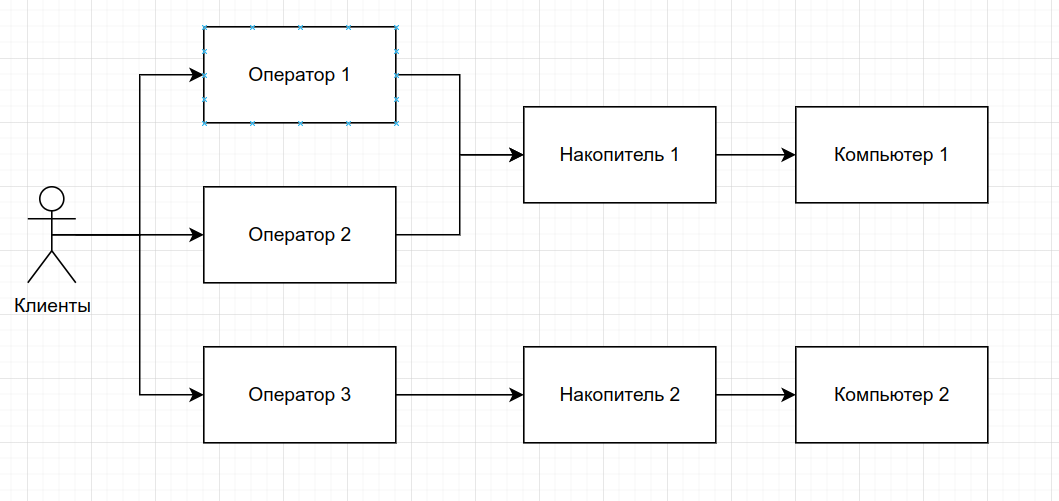
\includegraphics[width=0.7\linewidth]{inc/flow.png}
	\end{center}
	\caption{Структурная схема потока}
\end{figure}

\section{Демонстрация работы программы}

На рисунке 2 представлена демонстрация работы программы.

\begin{figure}[h]
	\centering
	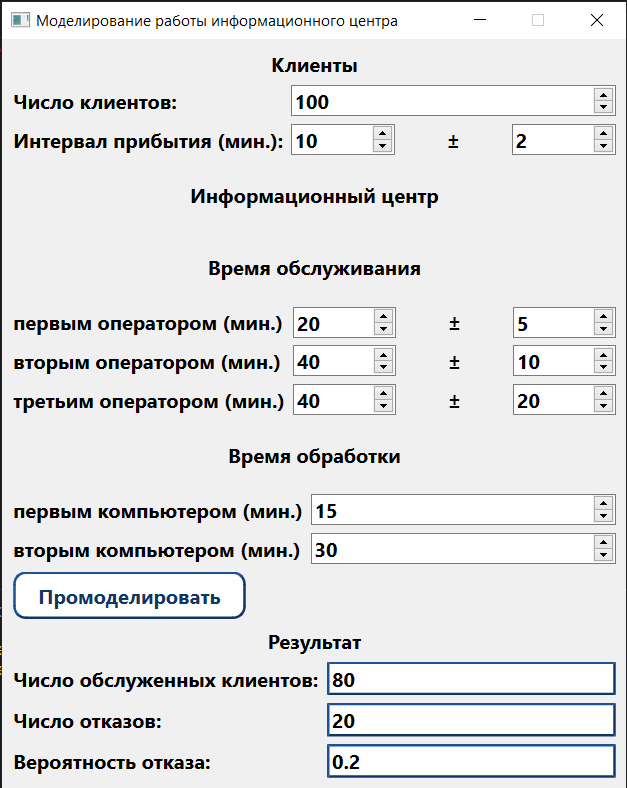
\includegraphics[width=0.7\linewidth]{inc/demo}
	\caption{Демонстрация работы программы}
	\label{fig:demo}
\end{figure}


